\section{Architettura}

Per l'architettura dell'applicativo da sviluppare si è deciso di utilizzare
\textit{Model-View-ViewModel}, derivato da \textit{Model-View-Controller}.

\subsection{Viste}
% TODO: Viste non nel senso del pattern
Per garantire l'uniformità e la riusabilità di tutti i componenti delle varie
viste si è deciso di utilizzare per tutti la stessa struttura.

\subsubsection{Caratterizzazione di una vista}
Una vista è caratterizzata da:
\begin{itemize}
  \item Tipo di grafico (scatterplot, parallel coordinates, ecc...).
  \item Impostazioni di rendering.
  \item Associazione degli assi alle dimensioni del grafico.
\end{itemize}

\subsubsection{Logica di Rendering}
\begin{itemize}
  \item Renderer: componente che si occupa tramite WebGL di effettuare il
    render del grafico, esso opera su il dataset già preparato per il render
    (ad esempio mappati come punti 2 dimensionali nello scatterplot) sulle sue
    impostazioni specifiche di rendering (ad esempio lunghezza degli assi x ed
    y nello scatterplot).
  \item Mapper: componente che si occupa di trasformare il dataset generale nel
    dataset preparato per il render.
\end{itemize}
Tutte queste generalizzazioni sono presenti all'interno di
\texttt{src/genericview}.

\begin{figure}[h!]
  \centering
  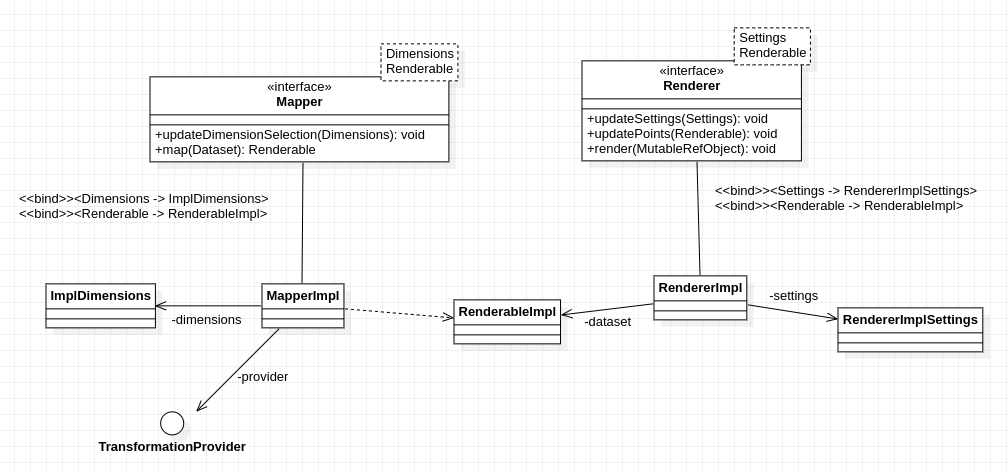
\includegraphics[scale=0.65]{../../assets/classi_uml/modelvista.png}
  \caption{Esempio di implementazione di una vista di tipo \texttt{Impl}.}
\end{figure}

\subsubsection{Interazione con l'utente}
L'utente deve poter interagire con l'applicazione per poter modificare
preferenze del grafico specifico, quindi si utilizza mvvm per modellare questa
interazione.

\begin{figure}[h!]
  \centering
  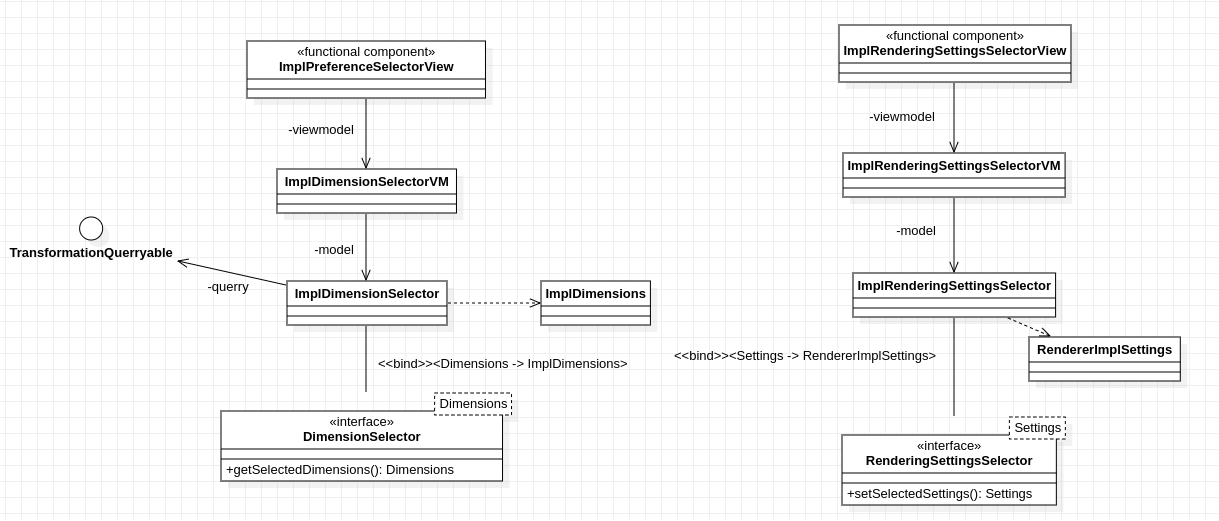
\includegraphics[scale=0.55]{../../assets/classi_uml/modelinterazione.png}
  \caption{Esempio di implementazione dell'interazione di tipo \texttt{Impl}.}
\end{figure}

% \subsection{Diagrammi dei package}
% \subsection{Diagrammi delle classi}

% \subsubsection{View}

% \begin{figure}[h!]
    % \centering
    % 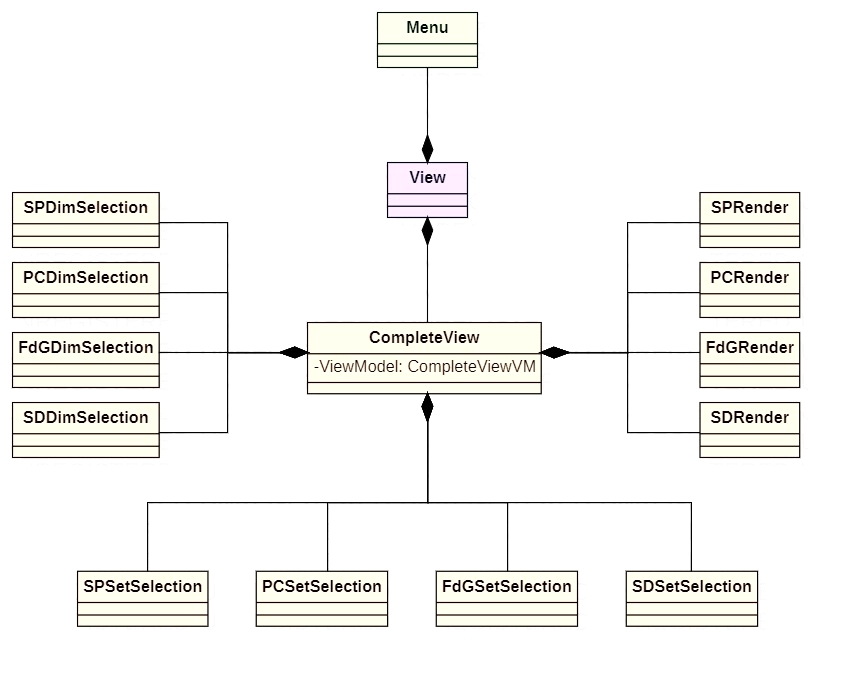
\includegraphics[scale=0.75]{../../assets/classi_uml/View.jpg}
    % \caption{Diagramma delle classi - View}
% \end{figure}
% \newpage
% \subsubsection{Model}

% \begin{figure}[h!]
    % \centering
    % 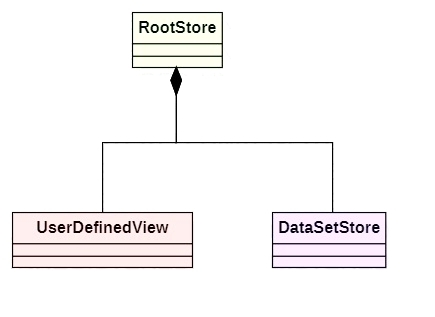
\includegraphics[scale=0.75]{../../assets/classi_uml/Model.jpg}
    % \caption{Diagramma delle classi - Model}
% \end{figure}

% \subsection{Diagrammi di sequenza}
